\documentclass{beamer}
\usepackage{standalone}

\usepackage{stmaryrd}

\usepackage[hyperref=auto,style=alphabetic]{biblatex}
\addbibresource{kwarc.bib}
\usepackage{appendixnumberbeamer}
\usepackage{tikz}
\usetikzlibrary{arrows.meta}

\usetheme{Pittsburgh}
\setbeamertemplate{footline}[frame number]
\setbeamertemplate{navigation symbols}{}
\usecolortheme{beaver}
\setbeamertemplate{frametitle}[default][left]
\setbeamersize{text margin left=3em}

\usepackage{utils/colors}
\usepackage[forbeamer]{utils/basic}

\title{GLIF: A Declarative Framework for Symbolic Natural Language Understanding}

\author{\underline{Jan Frederik Schaefer} \and Michael Kohlhase}
\institute{FAU Erlangen-N\"urnberg}
\date{\textbf{FCR 2020} \\ \textit{virtual event due to COVID-19} \\ September 22, 2020 }

\begin{document}
\frame\titlepage

\begin{frame}
    \frametitle{Method of Fragments}
    \only<1-2>{
        \centering
        \only<1>{\def\fraglevel{0}}
        \only<2>{\def\fraglevel{1}}
        \includestandalone{fig/montague-fragments}

        \begin{minipage}[t][2cm]{\textwidth}\vspace{1em}
            How do we get from messy language to formal logic?\\[0.5em]
            \emph{Montague}~\cite{Montague:efl70}: Look at a ``nice'' subset
            and map into logic.
        \end{minipage}
    }

    \only<3>{
        \centering
        \def\fraglevel{1}
        \includestandalone{fig/montague-fragments}
        
        \begin{minipage}[t][2cm]{0.6\textwidth}\vspace{1em}
            \str{Ahmed paints and Berta is quiet.}\\[0.5em]
            \str{Ahmed doesn't paint.}
        \end{minipage}\hfill
        \begin{minipage}[t][2cm]{0.39\textwidth}\vspace{1em}
            $p(a) \wedge q(b)$\\[0.5em]
            $\neg p(a)$
        \end{minipage}
    }

    \only<4>{
        \centering
        \def\fraglevel{2}
        \includestandalone{fig/montague-fragments}
        
        \begin{minipage}[t][2cm]{0.6\textwidth}\vspace{1em}
            \str{Every student paints and is quiet.}\\[0.5em]
            \str{Nobody paints.}
        \end{minipage}\hfill
        \begin{minipage}[t][2cm]{0.39\textwidth}\vspace{1em}
            $\forall x.s(x) \Rightarrow (p(x) \wedge q(x))$\\[0.5em]
            $\neg \exists x.p(x)$
        \end{minipage}
    }

    \only<5>{
        \centering
        \def\fraglevel{3}
        \includestandalone{fig/montague-fragments}

        \begin{minipage}[t][2cm]{0.6\textwidth}\vspace{1em}
            \str{Ahmed isn't allowed to paint.}\\[0.5em]
            \str{Ahmed and Berta must paint.}
        \end{minipage}\hfill
        \begin{minipage}[t][2cm]{0.39\textwidth}\vspace{1em}
            $\neg\lozenge p(a)$\\[0.5em]
            $(\square p(a)) \wedge \square p(b)$
        \end{minipage}
    }
\end{frame}


\begin{frame}
    \frametitle{Method of Fragments}
    If we only hand-wave, we gloss over problems:

    \hspace{2em}\str{Ahmed paints. He is quiet.}
    {$\quad\stackrel{?}{\leadsto}\quad$ \color{logicfont} $p(a)\wedge q(a)$}

    \vspace{1.5em}
    Specify:
    \begin{itemize}
        \item Grammar\com{fixes NL subset}
        \item Target logic
        \item Semantics construction\com{maps parse trees to logic}
    \end{itemize}

    \vspace{1.5em}
    On paper~\cite{Montague:tptoqi73}:\com{difficult to scale}

    \vspace{0.3em}\hspace{2em}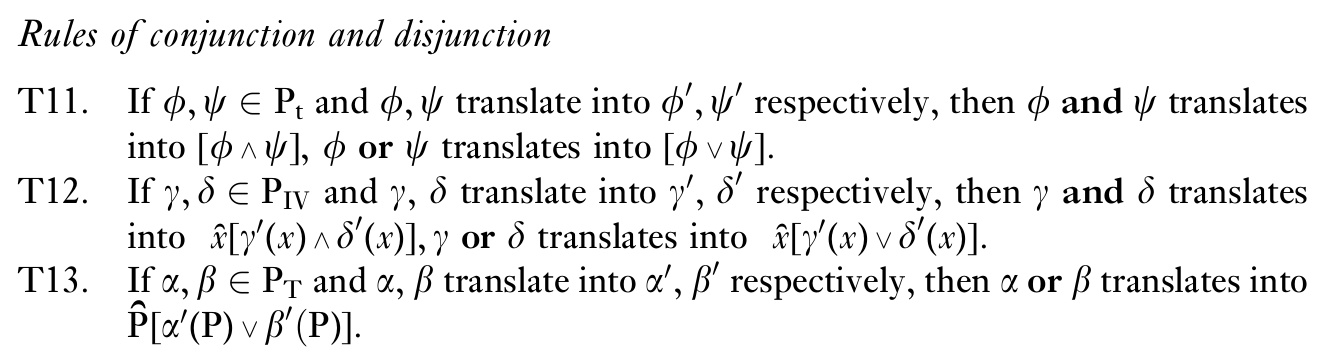
\includegraphics[trim=0 0 0 80,clip,width=0.8\textwidth]{fig/montague-tptoqioe.png}
    % \newcommand\VP{\text{\upshape\tiny VP}}
    % \hspace{2em}$\llbracket\text{\strplain{$P_{\VP}$ and $Q_{\VP}$}}\rrbracket_{\VP} = \lambda x. \llbracket\text{\strplain{$P_{\VP}$}}\rrbracket(x) \wedge \llbracket\text{\strplain{$Q_{\VP}$}}\rrbracket(x)$
\end{frame}

\begin{frame}
    \frametitle{GLIF: Grammatical Logical Inference Framework}
    \centering

    \parbox[t][1em][t]{\textwidth}{
        \centering\textit{
            \only<1-2>{We have a tool for this!}
            \only<3>{It combines existing tools.}
        }
    }

    \vspace{1.5em}
    \only<1-1>{\disablepart{sempragarrow}}
    \only<1-2>{\disablepart{includejupyter}}
    \only<1-2>{\disablepart{gfbox}\disablepart{mmtbox}\disablepart{elpibox}}
    \includestandalone[width=\textwidth]{fig/glif-architecture}

    \vspace{1.5em}
    \begin{minipage}[t][2cm]{\textwidth}
        \only<1-2>{
            \begin{tikzpicture}
                \node(str) at (-4,0) {\str{Ahmed and Berta paint.}};
                % REQUIRES \usepackage{tikz-qtree}
                \node(ast) at (0,0) {\color{nlfont!50!logicfont}
                    \resizebox{1.5cm}{!}{\tikzset{edge from parent/.append style={very thick}}
                    \Tree [ .\textbf{mkS} [ .\textbf{andNP} [ \textbf{Ahmed} \textbf{Berta} ] ] \textbf{paint} ]
                    }};
                \node(log) at (2.8,0) {\color{logicfont}$p(a) \wedge p(b)$};
                \draw[-{Straight Barb[length=6.3,width=5.0]},gray] (str) -- (ast);
                \draw[-{Straight Barb[length=6.3,width=5.0]},gray] (ast) -- (log);
            \end{tikzpicture}
        }
        \only<3>{
            \setlength{\arrayrulewidth}{1.0pt}
            \begin{tabular}{r@{\hskip3pt} l l}
                \vspace{0.1em} &\textbf{GF}   &{(= \textbf{grammar} framework)}\\
                \vspace{0.1em}+&\textbf{MMT}  &{(= \textbf{logic} framework)}\\
                \vspace{0.1em}+&\textbf{ELPI} &{(= \textbf{inference} framework)}\\
                \hline
                \\[-1em]
                =&\textbf{GLIF} &{(= \textbf{natural language understanding} framework)}\\
                \end{tabular}
        }
    \end{minipage}
\end{frame}


\begin{frame}[allowframebreaks,t]
    \frametitle{References}
    \printbibliography
\end{frame}



\end{document}
